\chapter[REVISÃO TEÓRICA]{REVISÃO TEÓRICA}
%---------------------------------------------------------------------------------------

% Muitos problemas de engenharia estão relacionados a geometrias complexas, em que o uso de um sistema de coordenadas cartesianas, cilíndricas ou esféricas não se mostra prático ou adequado. Exemplo placa com furo como na figura \ref{fig:placa_furo}.

% \begin{figure}[ht]
%     \centering
%     \includegraphics{fig/placa_furo.eps}
%     \caption{Placa com Furo}
%     \label{fig:placa_furo}
% \end{figure}

% Malhas cartesianas são exemplos de um método estruturado. Como características de uma malha estruturada, tem-se:

% \begin{itemize}
%     \item os pontos nodais são posicionados nas interseções das linhas coordenadas.
%     \item os pontos nodais interiores (que não estão posicionados nos contornos) possuem um número fixo de pontos nodais vizinhos.
%     \item os pontos nodais podem ser mapeados dentro de uma matriz, sua localização na malha e na matriz é fornecida por índices (comumente i,j em problemas 2d e i,j,k em problemas 3d).
% \end{itemize}

% Os métodos em CFD para geometrias complexas podem ser classificados em dois grupos:

% \begin{itemize}
%     \item malhas não-ortogonais (malhas curvilíneas) estruturadas
%     \item malhas não-estruturadas
% \end{itemize}

% Malhas não-ortogonais estruturadas (ou malhas coincidentes com o corpo / com a fronteira do domínio) são baseadas no mapeamento do "domínio de escoamento" sobre o "domínio computacional" com um formato simples, nota-se contudo, que encontrar um mapeamento viável pode se tornar complicado para geometrias complexas. Neste caso, pode-se recorrer à subdivisão do domínio em diferentes subregiões ou blocos, cada qual apresentando uma malha em separado que deverá ser unida corretamente aos seus vizinhos. Tem-se neste caso as malhas estruturadas por blocos.

% Uma generalização da técnica de malhas estruturadas por blocos é o caso de malhas não-estruturadas, para as quais cada bloco é formado por um único elemento (ou célula). Malhas não-estruturadas garantem uma flexibilidade geométrica ilimitada e são empregadas para escoamentos em geometrias complexas, sendo atualmente a mais empregada técnica em CFD industrial.

% \subsection{Vantagens do uso de malhas estruturadas}

% \begin{itemize}
%     \item obtenção de matrizes diagonais (devido à ordenação)
%     \item solvers mais fáceis de serem desenvolvidos e mais eficientes
%     \item equações governantes descritas de modo mais simples
% \end{itemize}

% \subsection{Desvantagens do uso de malhas estruturadas}
% \begin{itemize}
%     \item adaptabilidade para geometrias complexas
% \end{itemize}

% \subsection{Vantagens do uso de malhas não-ortogonais}
% \begin{itemize}
%     \item maior adaptabilidade para geometrias
%     \item obtenção de matrizes diagonais
%     \item emprego de solvers disponíveis para malhas estruturadas
% \end{itemize}

% \subsection{Desvantagens do uso de malhas não-rotogonais}
% \begin{itemize}
%     \item equações governantes apresentadas em forma mais complexas
%     \item apresentam maior tempo de geração (deviao ao mapeamento a ser realizado)
%     \item em alguns casos, o mapeamento pode ser impossível devido a complexidades geométricas
% \end{itemize}

% \subsection{Vantagens do uso de malhas não-estruturadas}
% \begin{itemize}
%     \item versatilidade, adaptabilidade para qualquer complexidade geométrica
%     \item facilidade de refino local de malha, para pontos de maior interesse (como regiões de recirculação, camadas-limite entre outras)
% \end{itemize}

% \subsection{Desvantagens do uso de malhas não-estruturadas}
% \begin{itemize}
%     \item maior complexidade na discretização
%     \item obtenção de matrizes não-diagonais que devem ser solucionadas por solvers mais gerais (dificuldades na ordenação dos dados)
% \end{itemize}

% \subsection{Conceitos de elementos e volumes de controle}

% O converito de elementos não é tradicionalmente usado no método de volumes finitos pois basta definir volumes de controle para a integração das equações governantes e posterior aproximações pertinentes ao processo de discretização.

% Os elementos são sempre definidos em função da malha criada pelo gerador de malhas, o elemento é um ente geométrico que cobre todo o domínio computacional sem superposição e sem pedaços nas fronteiras.

% Os volumes de controle são criados tendo-se por base os elementos criados. Existem duas classes básicas de métodos de determinação dos volumes de controle, baseadas na relatividade geométrica entre volumes e elementos:

% \begin{itemize}
%     \item Volumes centrado ou célula centrada (cell-centered): as informações (variáveis de interesse) são determinadas no centro (geométrico) do volume de controle, que coincide com o elemento de malha. Esta é a construção clássica de volumes finitos, em que os pontos de integração se localizam no centro das faces. \ref{fig:volume_centrado}
%     \item Volume de controle baseado no vértice (vertex-based control volumes): o volume de controle é construído com seu centro coincidente a um nó da malha, ou seja, a um vértice do elemento de malha. Cada volume de controle é constituído por partes (subvolumes de controle) dos elementos vizinhos, aos quais pertence o nó empregado como centro do volume, onde são armazanadas as informações. Uma metodologia para geração dos volumes, conhecida como método das medianas, consiste em ligar os centroides dos elementos aos pontos médios de suas faces. \ref{fig:volume_vertice}
% \end{itemize}

% \begin{figure}[ht]
%     \begin{subfigure}{.5\textwidth}
%         \centering
%         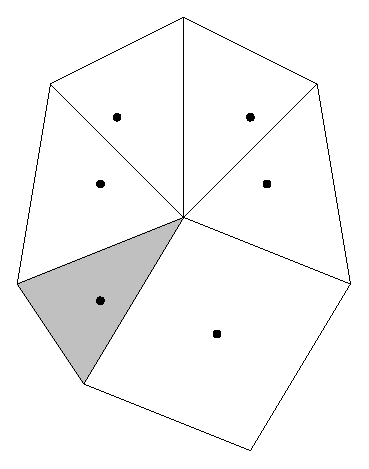
\includegraphics[width=.8\linewidth]{fig/volume_centrado.eps}
%         \caption{Volume Centrado}
%         \label{fig:volume_centrado}        
%     \end{subfigure}
%     \begin{subfigure}{.5\textwidth}
%         \centering
%         \includegraphics[width=.8\linewidth]{fig/volume_vertice.eps}
%         \caption[]{Volume Baseado no vértice}
%         \label{fig:volume_vertice}        
%     \end{subfigure}

%     \caption{Criação de Volumes de Controle}
%     \label{fig:volume-controle}
% \end{figure}


% \subsection{Acurácia Numérica}
% A acurácia numérica na área de dinâmica de fluídos computacional vem tornando-se muito importante na engenharia \cite{doi:10.1080/10407791003685155}. O método mais usado para resolver problemas de fluxo de fluidos é o método dos volumes finitos (FVM), que será discutido no capítulo \ref{Volumes Finitos}.

% O erro de discretização é uma classe de erros muito importante no FVM, que é o método usado nesse trabalho. Existem vários trabalhos cujo objetivo é estimar esse erro de discretização \cite{Muzaferija2014} \cite{Jasak1996} Existem várias maneiras de se estimar esse erro de discretização, esse erro pode ser usado para motivar o refinamento da malha de modo a se controlar o valor desse erro.

% Existem análises de vários esquemas de discretização que incluem a influência da qualidade da malha na solução devido a vários parâmetros dessa malha.

% Esse erro de discretização é também influenciado pelo tipo de células da malha. \cite{doi:10.1080/10407791003685155}

% Esse erro afeta os termos de convecção e difusão para diferentes formatos de volumes de controle, nesse trabalho será considerado apenas células triangulares pois são o tipo mais usado por poderem ser geradas com uma triangularização de Delaunay.

% O capítulo \ref{Volumes Finitos} apresenta o método dos volumes finitos (FVM) e a dedução para o erro de discretização do termo de convecção e difusão.

% De modo a se escrever as equações em um novo sistema de coordenadas é apresentado a teoria necessária para tal conversão começando no capítulo \ref{Transformação de Coordenadas} e depois, com a malha gerada, no capítulo \ref{Difusão de calor 2D em regime permanente}.

% A geração de malhas não estruturadas é mostrada no capítulo \ref{Malhas não estruturadas}.
